\documentclass[10pt,onecolumn,twoside,letterpaper]{article}
\usepackage[text={7in,9.5in},centering]{geometry}
\usepackage[spanish,es-nodecimaldot]{babel}

\usepackage{hyperref}

\usepackage{multicol}
\usepackage{amsmath,amssymb,amsthm}

\usepackage{harvard}% bibliographystyle: apsr, agsm, dcu, kluwer, nederlands
\newcommand{\myreferences}{../../../doc/review/review/library}
\usepackage{graphicx}
\graphicspath{{../../../doc/images/}}
\usepackage{amssymb}
\usepackage{fancyhdr}
\usepackage{color}
\usepackage{colortbl}
\definecolor{gray}{cmyk}{0.0,0.0,0.0,0.60}

\usepackage{float}

%\usepackage{auto-pst-pdf}
%\usepackage{pst-all}

%\usepackage[numbered]{mcode}
%\usepackage{lipsum}

\pagestyle{fancy}
\fancyhf{}
\fancyhead[RO]{\small{\textcolor{gray}{\textsc{Hacia un framework de locomoci\'on b\'ipeda, evolutiva y flexible}}}}
\fancyhead[LO]{
\includegraphics[scale=0.05]{unlogo.png}}
\fancyhead[LE]{
\includegraphics[scale=0.05]{unlogo.png}\quad\small{\textcolor{gray}{\textsc{Control Inteligente 2015-01}}}}
\fancyhead[RE]{\small{\textcolor{gray}{\textsc{TALLER 01}}}}
\fancyfoot[CO,CE]{\thepage}
\fancyfoot[LO,RE]{\scriptsize{\textcolor{gray}{\emph{Version 0.1}}}}

\title{\vspace{-0.8cm}
\includegraphics[scale=0.12]{unescudobn.png}\\\vspace{-0.0cm}
  \LARGE \textbf{Taller 2 - }}
\author{J.A. Castillo-Le\'on\thanks{jacastillol@unal.edu.co} \and Ronny Gelleschus\thanks{rgelleschus@unal.edu.co}}
\date{}

\begin{document}
\maketitle
\begin{abstract}\noindent\small\textit{En el siguiente documento se describen...}
\end{abstract}\vspace{1cm}
\par{\bf \large Punto 1:} Considere el conjuto difuso $\mathcal{C}$ definido por su funci\'on de pertenencia $\mu_c(x):\mathbb{R}\to[0,1]:$ con $\mu_c=1/(1+(x-1)^2)$. Calcule el $\alpha$-corte de $\mathcal{C}$ para $\alpha=0.5$, $\mathcal{A}_{0.5}$ (ver Figura \ref{fig:Acut05}).\\
Soluci\'on: Como se propone en \cite{Babuska1999}, $\mathcal{A}_{0.5}=\left\{x|\mu_c(x)\geq0.5\right\}$ con $x\in\mathbb{R}$. A continuaci\'on se demuestra que $\mu(x)\,\geq\,0.5\,\forall x \in [0,2]$,
\begin{align*}\small
  \mu_c&=1/(1+(x-1)^2)\geq 0.5 \tag{intercambiando}
  \\0.5&\leq 1/(1+(x-1)^2) \tag{observar que: $1+(x-1)^2\geq 1\,\forall x\in\mathbb{R}$}
  \\0.5(1+(x-1)^2)&\leq 1 \tag{reduciendo}
  \\(x-1)^2-1&\leq 0 \tag{reduciendo}
  \\x(x-2)&\leq 0 
\end{align*}
Notar primero que $x\leq 0\,\forall x\in(-\infty,0]$ y segundo que $(x-2)\leq0\,\forall x\in(-\infty,2]$. Usando el producto de los dos intervalos con la restricci\'on se concluye que $x\in [0,2]$.
\begin{figure}[H]
 \centering
 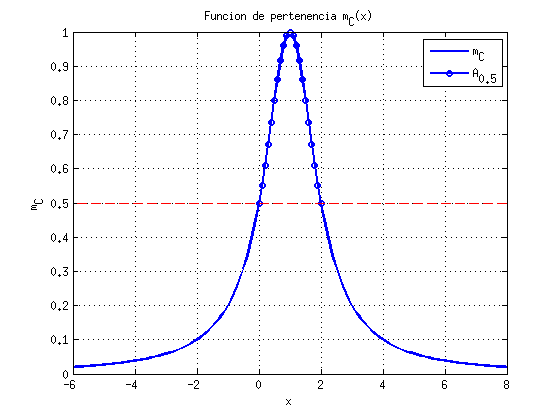
\includegraphics[scale=0.6]{A_05.png}
 \caption{Conjunto $\mathcal{A}_{0.5}$}
 \label{fig:Acut05}
\end{figure}
\par{\bf \large Punto 2:} Considere los conjutos difusos $\mathcal{A}$ y $\mathcal{B}$, tales que el $core(\mathcal{A})\cap core(\mathcal{B})\,=\,\emptyset$
\par{\bf 2.1: ¿Es el conjuto difuso $\mathcal{C}\,=\,\mathcal{A}\cap \mathcal{B}$ normal? Por qu\'e?}\\
Por definici\'on seg\'un \cite{Babuska1999}, $core(\mathcal{A})=\left\{x|\,\mu_A=1\right\}$, $supp(\mathcal{A})=\left\{x|\,\mu_A>0\right\}$ y $\mathcal{A}_{\alpha}=\left\{x|\,\mu_A\geq\alpha\right\}$, por lo tanto al definir los conjutos por comprens\'ion o por propiedad, $\emptyset=core(\mathcal{A})\cap core(\mathcal{B})=\left\{x|\,\mu_A=1\right\}\wedge\left\{x|\,\mu_B=1\right\}=\left\{x|\,\mu_A=1\,\wedge\,\mu_B=1\right\}=core(\mathcal{A}\cap\mathcal{B})$, por lo tanto se puede concluir que $\mathcal{C}$ no es normal.\\
\par{\bf 2.2: ¿Es el conjuto difuso $\mathcal{C}\,=\,\mathcal{A}\cap \mathcal{B}$ convexo o no convexo? Por qu\'e?}\\
El conjunto difuso $\mathcal{C}$ puede ser tanto convexo como no convexo y depende de las caracter\'isticas de $\mathcal{A}$ y $\mathcal{B}$, a continuaci\'on se describen dos ejemplos para soportar la afirmaci\'on anterior, para ello se toma la definici\'on: \emph{Un conjunto difuso} $\mathcal{A}$ \emph{es convexo si} $\forall \alpha\in[0,1]$, \emph{el intervalo de corte} $\mathcal{A}_\alpha$ \emph{es convexo}. De la misma forma, \emph{Un conjunto difuso} $\mathcal{A}$ \emph{es no convexo si} $\exists \alpha\in[0,1]$, \emph{tal que ese intervalo de corte} $\mathcal{A}_\alpha$ \emph{es no convexo}
\par \textcolor{blue}{\texttt{Caso convexo:}} Suponga $\mathcal{A}$ y $\mathcal{B}$ son convexos, por lo tanto $\mathcal{A}\cap\mathcal{B}$ es convexo.
\par \textcolor{blue}{\texttt{Caso no convexo:}} Suponga $\mathcal{A}$ es no convexo tal que $\exists{\alpha}_{nc}|\,(\alpha_{nc}\in(0,1))\wedge(\mathcal{A}_{\alpha_{nc}}\text{ es no convexo})$ y $\mathcal{B}$ es convexo tal que $\mathcal{A}_{\alpha_{nc}}\cap\mathcal{B}_{\alpha_{nc}}\neq\emptyset$ y a su vez es no convexo, por lo tanto $\mathcal{A}\cap\mathcal{B}$ es no convexo.
\begin{figure}[H]
 \centering
 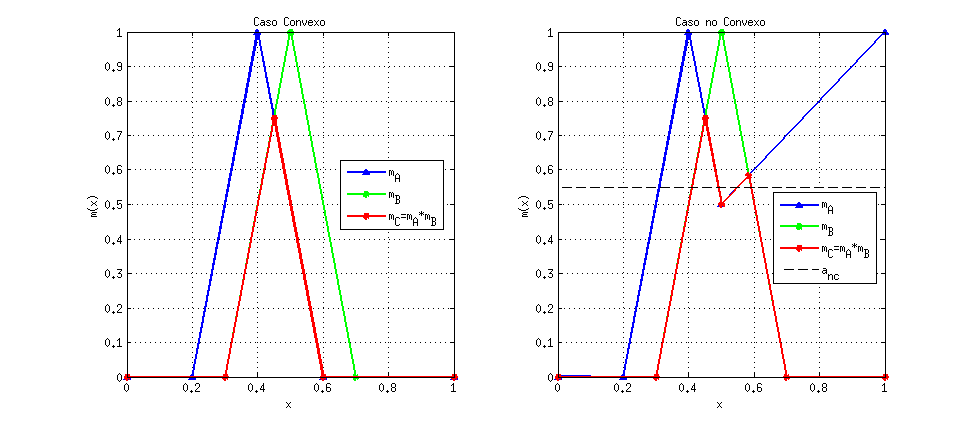
\includegraphics[scale=0.6]{CnvxOrNotCnvx.png}
 \caption{Conjunto convexo $\mathcal{C}$(Izq). Conjunto no convexo $\mathcal{C}$(Der)}
 \label{fig:CnvxOrNotCnvx}
\end{figure}
\par{\bf 2.3: Cardinalidad y condiciones para $card(\mathcal{C})>0$}\\
\par Seg\'un \cite{Babuska1999}, \emph{Cardinalidad de un conjunto difuso finito $\mathcal{A}=\left\{x_1,x_2,\ldots,x_n\right\}$, $card(\mathcal{A})$ como $\left|\mathcal{A}\right|=\sum_{i=1}^n\mu_A(x_i)$}. Se puede decir que si $\mathcal{A}$ es finito, $supp(\mathcal{A})\neq\emptyset$ entonces $card(\mathcal{A})>0$ y al igual $\mathcal{B}$ es finito, $supp(\mathcal{B})\neq\emptyset$ entonces $card(\mathcal{B})>0$, adem\'as si $\mathcal{A}\cap\mathcal{B}\neq\emptyset$ se puede afirmar que por lo anterior $card(\mathcal{A})>0$.
\par{\bf \large Punto 3:} Calcular las proyecciones de $\mathcal{A}$ sobre $X$ y $Y$.
\begin{equation}
  \label{eq:ej3}
  \mathcal{A}\,=\,\left\{0.2/(x_1,y_1),0.3/(x_1,y_2),0.6/(x_2,y_1),0.8/(x_2,y_2)\right\}
\end{equation}
aplicanado la proyecci\'on sobre el eje $X$, $proj_X(\mathcal{A})=\left\{max(\mu_1,\mu_2)/x_1,max(\mu_3,\mu_4)/x_2\right\}$, remplazando $proj_X(\mathcal{A})=\left\{max(0.2,0.3)/x_1,max(0.6,0.8)/x_2\right\}$ y simplificando $proj_X(\mathcal{A})=\left\{0.3/x_1,0.8/x_2\right\}$. De la misma manera se opera con el eje $Y$ obteniendo $proj_Y(\mathcal{A})=\left\{0.6/y_1,0.8/y_2\right\}$  (ver Figura \ref{fig:ProyA}.a).
\par{\bf \large Punto 4:} Calcular la extensi\'on cil\'indrica de $\mathcal{A}$ sobre $X\times Y$.
\begin{equation}
  \label{eq:ej3}
  \mathcal{A}\,=\,\left\{0.3/(x_1),0.5/(x_2)\right\}
\end{equation}
aplicanado la extensi\'on cil\'indrica $ext_Y(\mathcal{A})=\left\{0.3/(x_1,y),0.5/(x_2,y)\mid y\in Y\right\}$ (ver Figura \ref{fig:ProyA}.b).
\begin{figure}[H]
 \centering
 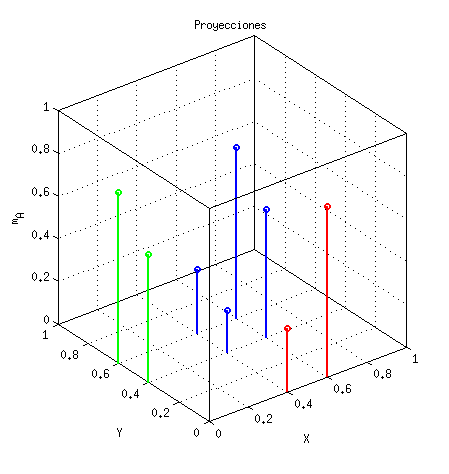
\includegraphics[scale=0.6]{ProjA.png}
 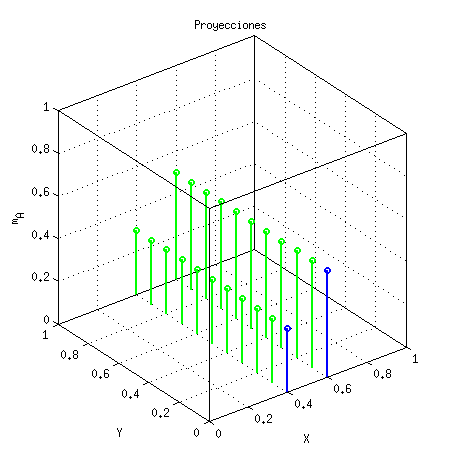
\includegraphics[scale=0.6]{ExtA.png}\\
 a)\hspace{7.5cm}b)
 \caption{a) Proyecci\'on sobe el eje $X$ y sobre el eje $Y$, b) Extensi\'on cilindrica sobre el plano $X\times Y$}
 \label{fig:ProyA}
\end{figure}
\par{\bf \large Punto 5:} Definici\'on de etiqueta ling\"uistica y variable ling\"uistica\\
En un ejemplo cuando se habla de \emph{altura}, se puede definir a la variable ling\"uistica $x$ como la \emph{altura}. Los ``valores'' que puede tomar $x$ est\'an dentro de un conjuto de etiquetas ling\"uistica, como por ejemplo \{\emph{alto, medio, bajo}\}.
\par \textcolor{blue}{\texttt{Etiqueta Ling\"uistica:}} Una etiqueta ling\"uistica representa un conjuto difuso caracterizado por una funci\'on de pertenencia o membrec\'ia. Es una forma de discretizar el universo discurso de una variable ling\"uistica $x$.
\par \textcolor{blue}{\texttt{Variable Ling\"uistica:}} Se puede decir, el conjuto (o uni\'on) que representa a todas las etiquetas ling\"uisticas y reproduce el universo de discurso describe a su vez a la variable ling\"uistica.
\par{\bf \large Punto 6:} Dada una relacion difusa $\mathbf{R}:X\times Y\to[0,1]$:\\
\begin{equation*}
  \label{eq:relation}
  R\,=\,
  \begin{array}{cccc}
    &y_1&y_2&y_3\\
    x_1&0.7&0.3&0.1\\
    x_2&0.4&0.8&0.2\\
    x_3&0.1&0.2&0.9
  \end{array}
\end{equation*}
y un conjuto difuso $\mathcal{A}\,=\,\left\{0.1/x_1,1/x_2,0.4/x_3\right\}$, determinar $\mathcal{B}\,=\,\mathcal{A}\circ R$, primero con el operador $max-min$ y luego con el operador $max-prod$.
\par \textcolor{blue}{\texttt{Operador max-min:}} 
\begin{equation*}
  \label{eq:relation}
  min(\mathcal{A},R)\,=\,min(\left[
  \begin{array}{ccc}
    0.1&0.1&0.1\\
    1.0&1.0&1.0\\
    0.4&0.4&0.4\\
  \end{array}\right],\left[
  \begin{array}{ccc}
    0.7&0.3&0.1\\
    0.4&0.8&0.2\\
    0.1&0.2&0.9\\
  \end{array}\right])\,=\,\left[
  \begin{array}{ccc}
    0.1&0.1&0.1\\
    0.4&0.8&0.2\\
    0.1&0.2&0.4
  \end{array}\right]
\end{equation*}
%begin{multicols}{2}
%\begin{figure}[H]
%  \centering
%  \includegraphics[scale=0.25]{3RLateralRobot.png}
%  \caption{Modelo Din\'amico General}
%  \label{fig:modelo}
%\end{figure}
%end{multicols}
%\nocite{*}
\bibliographystyle{nederlands}% apsr, agsm, dcu, kluwer, nederlands
\bibliography{\myreferences}
\end{document}
